\PassOptionsToPackage{dvipsnames}{xcolor}
\documentclass[11pt,aspectratio=169]{beamer}
% metadata
\newcommand{\github}{\href{https://github.com/c-uhs/turnover}{\texttt{https://github.com/c-uhs/turnover}}}
\title
[Risk group turnover in STI/HIV epidemics]
{Risk group turnover in STI/HIV epidemics}
%:\\mechanistic insights from transmission modeling}
\newcommand{\inst}[1]{\enspace\textsuperscript{#1}\thinspace}
\author[\github]
  %[Knight, Wang, Ma, Schwartz, Baral, Mishra]
  {\footnotesize
  Jesse Knight\inst{1},
  Linwei Wang\inst{1},
  Huiting Ma\inst{1},
  Sheree Schwartz\inst{2},
  Stefan Baral\inst{2},
  Sharmistha Mishra\inst{1}
}
\institute{
  \inst{1}MAP Centre for Urban Health Solutions, Unity Health Toronto\\
  \inst{2}Dept.~Epidemiology, Johns Hopkins Bloomberg School of Public Health
}
\newcommand{\logos}{
\begin{tabular}{*{6}{c}}
   
\includegraphics[height=0.75cm,valign=c]{nih-crop}
 & 
\includegraphics[height=0.95cm,valign=c]{cihr}
 & 
\includegraphics[height=0.90cm,valign=c]{jhu}
 & 
\includegraphics[height=0.55cm,valign=c]{map-cuhs}
 & 
\includegraphics[height=0.70cm,valign=c]{smh}
 & 
\includegraphics[height=0.70cm,valign=c]{uoft}
\end{tabular}
}
%\titlegraphic{\vspace{2em}\logos}
\date{2019 July 17\\[1em]\scriptsize\theconference\\[-2em]}
% temporary paths
\newcommand{\outpath}{../../outputs}
\newcommand{\figpath}{\outpath/paper/sit/figs/}
\newcommand{\tikzpath}{\outpath/tikz/}
\newcommand{\datapath}{\outpath/paper/sit/data/}
% front matter
\makeatletter
\def\abbrfootnote{\gdef\@thefnmark{}\@footnotetext}
\makeatother
% enumerate & itemize
\usepackage{enumitem}
% references
\bibliographystyle{plainnat}
% fixing natbib & hyperref issues
\makeatletter
\def\bibinfo#1{%
  \@ifundefined{bibinfo@X@#1}%
  {\@firstofone}
  {\csname bibinfo@X@#1\endcsname}}
\makeatother
\newcommand*{\doi}[1]{DOI \href{https://doi.org/#1}{\texttt{#1}}}
% maths
\usepackage{bm,amsmath}
\usepackage{xstring}
\newcommand{\tarr}[1]{{\def\arraycolsep{3pt}[\begin{matrix}\StrSubstitute{#1}{,}{&}\end{matrix}]}} % TEMP
\newcommand{\es}{\enspace}
% tables
\usepackage{booktabs,caption,float}
\newcommand{\cellbox}[2]{\parbox[t]{#1}{\linespread{1}\selectfont{#2}}\vspace{3pt}}
% figures
\usepackage{graphicx,subcaption}
\graphicspath{
  {\tikzpath/turnover/}
  {\tikzpath/health/}
  {\tikzpath/tpaf-contexts/}
%  {\tikzpath/variants/}
  {\tikzpath/flows/}
  {\figpath/compare/}
  {\figpath/sensitivity/}
  {\figpath/flows/}
  {\outpath/paper/whatif/asso/figs/compare/}
  {\outpath/paper/whatif/mort/figs/compare/}
  {\outpath/paper/whatif/sirs/figs/compare/}
}
\captionsetup[sub]{size=footnotesize}
% footnotes
\usepackage[hang]{footmisc}
\setlength{\footnotesep}{\baselineskip}
\setlength{\footnotemargin}{1em}
% hyperlink
\usepackage[colorlinks]{hyperref}
% temp formatting
\renewcommand{\floatpagefraction}{0.8}
\interfootnotelinepenalty=10000
% appendix
\newcommand{\initappendix}{
  \appendix
  \numberwithin{figure}{section}
  \numberwithin{table}{section}
  \numberwithin{equation}{section}
  \renewcommand*{\thesection}{\Alph{section}}
}
%\logo{
\includegraphics[width=2cm]{isstdr-full.jpg}}
%%%%%%%%%%%%%%%%%%%%%%%%%%%%%%%%%%%%%%%%%%%%%%%%%%%%%%%%%%%%%%%%%%%%%%%%%%%%%%%%%%%%%%%%%%%%%%%%%%%%
\begin{document}
%%%%%%%%%%%%%%%%%%%%%%%%%%%%%%%%%%%%%%%%%%%%%%%%%%%%%%%%%%%%%%%%%%%%%%%%%%%%%%%%%%%%%%%%%%%%%%%%%%%%
\begin{frame}[noframenumbering]
  \titlepage
\end{frame}
%---------------------------------------------------------------------------------------------------
\begin{frame}[noframenumbering]{}{}
  \vfill
  {\usebeamerfont{frametitle}\usebeamercolor[fg]{frametitle}Disclosures}
  \vfill
  None.
  \vfill\vfill
  {\usebeamerfont{frametitle}\usebeamercolor[fg]{frametitle}Acknowledgements}
  \vfill
  \centering\scalebox{1}{\logos}
\end{frame}
%%%%%%%%%%%%%%%%%%%%%%%%%%%%%%%%%%%%%%%%%%%%%%%%%%%%%%%%%%%%%%%%%%%%%%%%%%%%%%%%%%%%%%%%%%%%%%%%%%%%
\begin{frame}[noframenumbering]{}{}
\tableofcontents
\end{frame}
%%%%%%%%%%%%%%%%%%%%%%%%%%%%%%%%%%%%%%%%%%%%%%%%%%%%%%%%%%%%%%%%%%%%%%%%%%%%%%%%%%%%%%%%%%%%%%%%%%%%
\section{Background}
% --------------------------------------------------------------------------------------------------
\begin{frame}{SIR Models \& Heterogeneity in Risk}
  \begin{minipage}{0.65\linewidth}
    \centering
    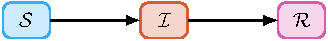
\includegraphics[width=0.4\linewidth]{health-states}
    \begin{itemize}
      \item SIR Model:
      \begin{itemize}
        \item $\S$ = susceptible, $\I$ = infectious, $\R$ = recovered
        \item e.g.\ HIV
      \end{itemize}
      \uncover<2->{
      \item 3 Risk Groups:}
      \begin{itemize}
        \uncover<2->{
        \item e.g.\ female sex workers, multiple partners, monogamous
        \item fundamentally changes epidemic dynamics~\cite{Stigum1994,Boily1997}}
        \uncover<5->{
        \item \parbox{2cm}{what about: }``retirement'' from sex work\\
              \hspace{2cm}``recruitment'' into sex work}
              \uncover<6->{\smash{\raisebox{0.7em}{$\Big\}$ \emph{Turnover}}}}
      \end{itemize}
    \end{itemize}
  \end{minipage}%
  \begin{minipage}{0.35\linewidth}
    \centering
    \uncover<2->{\scalebox{0.8}{%
      \begin{tikzpicture}
        \uncover<1->{\drawnodes}
        \uncover<3->{\drawentry}
        \uncover<4->{\drawexit}
        \uncover<6->{\drawturnover}
      \end{tikzpicture}}%
    \pseudocap{Risk groups}
    }
  \end{minipage}
\end{frame}
% --------------------------------------------------------------------------------------------------
\begin{frame}{Influence of Turnover in STI Epidemic Models}
  \begin{minipage}{0.65\linewidth}
    \uncover<2->{
    \textbf{Research Questions:}\\[1em]
    Influence of turnover on:}
    \begin{itemize}
      \uncover<3->{\item Equilibrium incidence \& prevalence by risk group}
      \uncover<4->{\item TPAF\,* of high risk group}
    \end{itemize}
    \vspace*{3em}\footnotesize
    \uncover<5->{
    *\,TPAF:~~\parbox[t]{\linewidth}{``Transmission Population Attributable Fraction''~\cite{Mishra2016}
    \\[0.5em]
    Proportion of cumulative new infections averted\\
    if transmission to\,/\,from that group is stopped.\\[0.5em]
    e.g.\ impact of perfect TasP in one group}}
  \end{minipage}%
  \begin{minipage}{0.35\linewidth}
    \centering
    \scalebox{0.8}{%
      \begin{tikzpicture}
        \drawnodes
        \drawentry
        \drawexit
        \drawturnover
      \end{tikzpicture}}%
    \pseudocap{Risk groups}
  \end{minipage}
\end{frame}
%%%%%%%%%%%%%%%%%%%%%%%%%%%%%%%%%%%%%%%%%%%%%%%%%%%%%%%%%%%%%%%%%%%%%%%%%%%%%%%%%%%%%%%%%%%%%%%%%%%%
\section{Methods}
%---------------------------------------------------------------------------------------------------
\begin{frame}{Illustrative Model of STI Transmission}
  \begin{minipage}{0.65\linewidth}
    \centering
    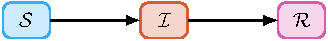
\includegraphics[width=0.4\linewidth]{health-states}
    \begin{itemize}
      \uncover<1->{
      \item SIR model:
      \begin{itemize}
        \item 1-sex
        \item proportional mixing
        \item same mortality across risk groups
      \end{itemize}}
      \uncover<2->{
      \item Risk group turnover:
      \begin{itemize}
        \item Rates ensure group sizes don't change:\\
        {\scriptsize 5\%~High Risk, 20\%~Medium Risk, 75\%~Low Risk}
        \item All rates equal among:   $\S,~\I,~\R$
        \item All rates scaled proportionally when varied
      \end{itemize}}
    \end{itemize}
  \end{minipage}%
  \begin{minipage}{0.35\linewidth}
    \centering
    \scalebox{0.8}{%
      \begin{tikzpicture}
        \drawnodes
        \drawentry
        \drawexit
        \drawturnover
      \end{tikzpicture}}%
    \pseudocap{Risk groups}
  \end{minipage}
\end{frame}
%---------------------------------------------------------------------------------------------------
\begin{frame}<1-2>[label=experiment]{Experiments: Influence of Turnover on Model Outputs}
  \begin{enumerate}
    \uncover<1,2,3>{
    \item Equilibrium outputs:
    \begin{itemize}
      \item \parbox{2cm}{\textbf{Vary:}}    Turnover magnitude
      \item \parbox{2cm}{\textbf{Compare:}} a) prevalence, b) incidence (by risk group, at equilibrium)
    \end{itemize}}
    \vspace{1em}
    \uncover<2,4>{
    \item TPAF after model fitting:
    \begin{itemize}
      \item \parbox{2cm}{\textbf{Fit:}}     Contact rates: High Risk; and Low Risk
      \item \parbox{2cm}{\textbf{Targets:}} Prevalence: 25\% in High Risk; and 5\% in Low Risk
      \item \parbox{2cm}{\textbf{Vary:}}    No-turnover vs Turnover
      \item \parbox{2cm}{\textbf{Compare:}} a) Fitted contact rates, b) TPAF of high risk group
    \end{itemize}}
  \end{enumerate}
\end{frame}
%%%%%%%%%%%%%%%%%%%%%%%%%%%%%%%%%%%%%%%%%%%%%%%%%%%%%%%%%%%%%%%%%%%%%%%%%%%%%%%%%%%%%%%%%%%%%%%%%%%%
\section{Results}
% --------------------------------------------------------------------------------------------------
\againframe<3>[noframenumbering]{experiment}
%---------------------------------------------------------------------------------------------------
\begin{frame}{Turnover decreases high risk group equilibrium prevalence}
  \begin{minipage}{0.45\linewidth}
    \centering
    \begin{tikzpicture}
      \node[anchor=south west] at (0,0) {\includegraphics[width=0.9\linewidth]{{1d-prevalence-high-tau=0.1}.pdf}};
      \only<3-4>{\draw[arrow=C2,<-] (1.75,4.35) -- ++(0,-1);}
      \only<5- >{\draw[arrow=C2,<-] (5.60,1.40) -- ++(0,+1);}
    \end{tikzpicture}
    \vspace{-1em}
    \pseudocap{High risk prevalence vs turnover}
  \end{minipage}%
  \begin{minipage}{0.55\linewidth}
    \raggedright
    \begin{tikzpicture}
      \only<2- >{\drawflownodes}
      \only<3- >{\node[right = 2.5 cm of m] {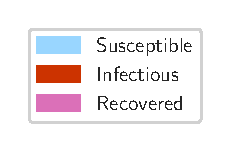
\includegraphics[width=0.4\linewidth]{flows-legend}};}
      \only<3-4>{\drawflowhigh{1}\drawflowpiehigh{low}}
      \only<4  >{\drawflowlow {1}\drawflowpielow {low}}
      \only<5- >{\drawflowhigh{3}\drawflowpiehigh{high}\drawflowlow{3}\drawflowpielow{high}}
    \end{tikzpicture}
  \end{minipage}
  \\[1em]
  \uncover<6->{\emph{Turnover causes a net movement of infected: high $\bm{\rightarrow}$ low risk}} 
\end{frame}
%---------------------------------------------------------------------------------------------------
\begin{frame}{Turnover increases low-risk equilibrium prevalence \uncover<3->{\color{C2}\dots at first}}
  \begin{minipage}{0.45\linewidth}
    \centering
    \begin{tikzpicture}
    \only<1-2>{\node[anchor=south west] at (0,0) {\includegraphics[width=0.9\linewidth]{{1d-prevalence-low-tau=0.1-trend}.pdf}};}
    \only<3- >{\node[anchor=south west] at (0,0) {\includegraphics[width=0.9\linewidth]{{1d-prevalence-low-tau=0.1-both}.pdf}};}
    \only<2  >{\draw[arrow=C2,<-] (1.75,1.4) -- ++(0,+1);}
    \only<3- >{\draw[arrow=C2,<-] (5.60,2.85) -- ++(0,+1);}
    \end{tikzpicture}
    \vspace{-1em}
    \pseudocap{Low risk prevalence vs turnover}
  \end{minipage}%
  \begin{minipage}{0.55\linewidth}
    \raggedright
    \begin{tikzpicture}
    \drawflownodes
    \node[right = 2.5 cm of m] {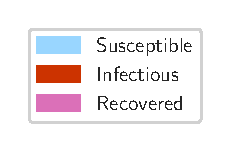
\includegraphics[width=0.4\linewidth]{flows-legend}};
    \only<2  >{\drawflowhigh{1}\drawflowpiehigh{low}\drawflowlow{1}\drawflowpielow{low}}
    \only<3- >{\drawflowhigh{3}\drawflowpiehigh{high}\drawflowlow{3}\drawflowpielow{high}}
    \end{tikzpicture}
  \end{minipage}
  \\[1em]
  \uncover<4->{\emph{High turnover reduces prevalence in all groups}}
  \uncover<5->{\emph{\dots but why?}}
\end{frame}
% --------------------------------------------------------------------------------------------------
\begin{frame}{Two competing effects of turnover on incidence}
  \begin{minipage}{0.45\linewidth}
    \centering
    \begin{tikzpicture}
      \node[anchor=south west] at (0,0) {\includegraphics[width=0.9\linewidth]{{1d-incidence-all-tau=0.1}.pdf}};
    \end{tikzpicture}
    \vspace{-1em}
    \pseudocap{Overall incidence vs turnover}
  \end{minipage}%
  \begin{minipage}{0.55\linewidth}
    \begin{itemize}
      \item<2-> Turnover $\bm\uparrow$ proportion who are infectious
      \begin{itemize}
        \item<4-> Dominates at low turnover (A)
        \item<5-> Incidence $\bm\uparrow$
      \end{itemize}
      \vspace{1em}
      \item<3-> Turnover $\bm\downarrow$ contact rate among infectious
      \begin{itemize}
        \item<6-> Dominates at high turnover (B)
        \item<7-> Incidence $\bm\downarrow$
      \end{itemize}
    \end{itemize}
    \vspace{1em}
    \footnotesize
    \uncover<8->{(explains low risk prevalence decline with high turnover)}
  \end{minipage}
  \\[1em]
  \uncover<9->{\parbox{0.5\linewidth}{\emph{Low turnover: $\bm\uparrow$ incidence}}}%
  \uncover<10->{\parbox{0.5\linewidth}{\emph{High turnover: $\bm\downarrow$ incidence}}}%
\end{frame}
%---------------------------------------------------------------------------------------------------
\againframe<4>[noframenumbering]{experiment}
%---------------------------------------------------------------------------------------------------
\begin{frame}[t]{Turnover makes it ``harder'' to observe a high prevalence ratio}
\newcommand{\uin}[2]{\uncover<####1->{\input{data/####2}}}
  \centering
  \begin{tabular}{llcc}
    \toprule
                 &           &          No turnover           &            Turnover            \\
    \midrule
    Prevalence   & High risk &       \uin{2}{notu-f-P-H.txt}  &       \uin{2}{turn-f-P-H.txt}  \\
                 & Low risk  &       \uin{2}{notu-f-P-L.txt}  &       \uin{2}{turn-f-P-L.txt}  \\
                 & Ratio     &       \uin{2}{notu-f-P-R.txt}  &       \uin{2}{turn-f-P-R.txt}  \\
    \midrule
    Contact rate & High risk &       \uin{3}{notu-f-C-H.txt}  &       \uin{4}{turn-f-C-H.txt}  \\
                 & Low risk  &       \uin{3}{notu-f-C-L.txt}  &       \uin{4}{turn-f-C-L.txt}  \\
                 & Ratio     & \emph{\uin{3}{notu-f-C-R.txt}} & \emph{\uin{4}{turn-f-C-R.txt}} \\
    \bottomrule
  \end{tabular}
  \\[1em]\raggedright
  \uncover<5->{\emph{To observe the same prevalence ratio:\\
      \hspace{1em}Risk heterogeneity must be higher with turnover than without}}\\
  \uncover<6->{\emph{\hspace{1em}(overcome ``homogenizing'' effect of turnover)}}
\end{frame}
% --------------------------------------------------------------------------------------------------
\begin{frame}[t]{TPAF of high risk group is higher with turnover than without}
  \begin{minipage}{0.45\linewidth}
    \centering
    \visible<1->{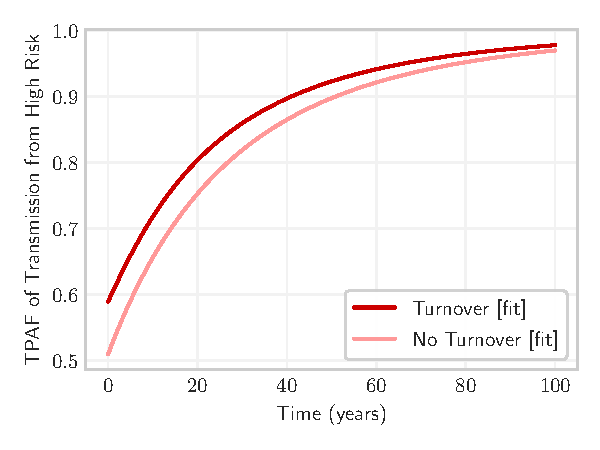
\includegraphics[width=0.9\linewidth]{tpaf-tpaf-high-all-fit}}\\[-0.5em]
  \end{minipage}%
  \begin{minipage}{0.55\linewidth}
    \footnotesize
    TPAF $\approx$ impact of perfect TasP in one group\\[1em]
    \normalsize
    \begin{itemize}
      \item<2-> Risk heterogeneity (contact rate ratio)\\is higher with turnover
      \item<3-> Impact of reaching high risk group\\is higher with turnover
    \end{itemize}
    \vspace{1em}
  \end{minipage}
  \\[1em]
  \uncover<4->{\emph{TPAF of high risk group may be underestimated if turnover is not modelled}}
\end{frame}
%%%%%%%%%%%%%%%%%%%%%%%%%%%%%%%%%%%%%%%%%%%%%%%%%%%%%%%%%%%%%%%%%%%%%%%%%%%%%%%%%%%%%%%%%%%%%%%%%%%%
\section{Conclusion}
%---------------------------------------------------------------------------------------------------
\begin{frame}{Implications}{}
  \newcommand{\cnum}[1]{\Large\textcircled{\small{####1}}}
  \begin{enumerate}
    \uncover<2->{
    \item[] Limitations:
    \begin{itemize}
      \item Results shown here conditional on model structure, assumptions, and parameters
    \end{itemize}}
    \vspace{1em}
    \uncover<3->{
    \item[\cnum{1}] \color{C2} Turnover influences equilibrium prevalence \& incidence
    \begin{itemize}
      \item Core prevalence always decreases (before fitting)
      \item Overall effect varies with context
    \end{itemize}}
    \vspace{0.5em}
    \uncover<4->{
    \item[\cnum{2}] \color{C2} TPAF of high risk group may be underestimated if turnover is not modelled
    \begin{itemize}
      \item Prevalence ratios we observe are likely \textit{in spite of} homogenizing effect of turnover
    \end{itemize}}
  \end{enumerate}
\end{frame}
% --------------------------------------------------------------------------------------------------
\begin{frame}[noframenumbering]{Thank you}
  \begin{minipage}{0.45\linewidth}
    \raggedleft
    \begin{tikzpicture}
      \drawflownodes\drawflowhigh{2}\drawflowlow{2}\drawflowpiehigh{low}\drawflowpielow{low}
    \end{tikzpicture}
  \end{minipage}%
  \hspace{0.1\linewidth}%
  \begin{minipage}{0.45\linewidth}
    \raggedright
    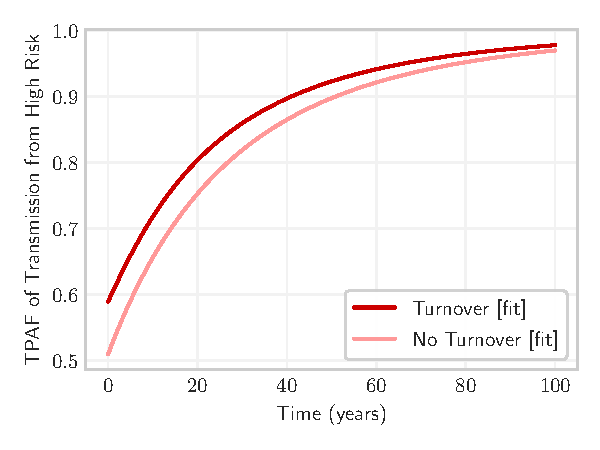
\includegraphics[width=0.8\linewidth]{tpaf-tpaf-high-all-fit}
  \end{minipage}
  \\[2em]\centering\logos
\end{frame}
% --------------------------------------------------------------------------------------------------
\begin{frame}[noframenumbering]{References}
  \nocite{Zhang2012,Alam2013,Henry2015}
  \printbibliography
\end{frame}
%%%%%%%%%%%%%%%%%%%%%%%%%%%%%%%%%%%%%%%%%%%%%%%%%%%%%%%%%%%%%%%%%%%%%%%%%%%%%%%%%%%%%%%%%%%%%%%%%%%%
\end{document}
%%%%%%%%%%%%%%%%%%%%%%%%%%%%%%%%%%%%%%%%%%%%%%%%%%%%%%%%%%%%%%%%%%%%%%%%%%%%%%%%%%%%%%%%%%%%%%%%%%%%
